\subsubsection{Besalisk}
\vspace{-2\baselineskip}
\begin{flushright}	
    \begin{tabular}{|l|r|}
        \textbf{Type} & Reptile \\
        \textbf{Planete} & Ojom \\
        \textbf{Langage} & Basic \\
        \textbf{Orientation} & Neutre\\
    \end{tabular}
\end{flushright}
\vspace{-3\baselineskip}
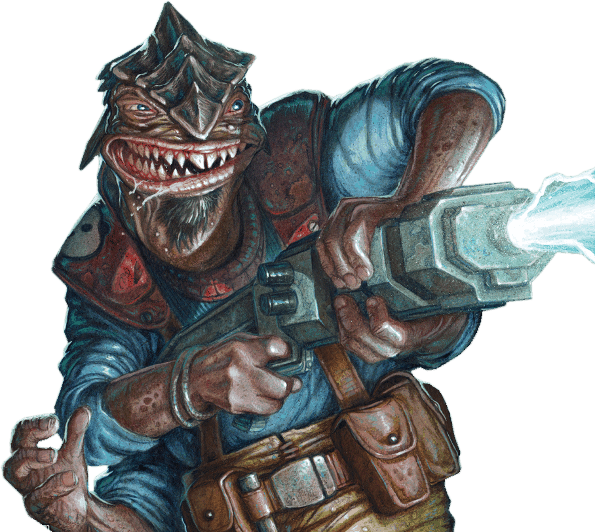
\includegraphics[width=8cm]{img/personnages/races/besalisk.png}
 
Trapus, les besalisks ont des bras très imposants, une crete osseuses au sommet du crâne (quelques petites plumes y logent). Reptiles bipedes, les mâles ont 4 bras, les deux supérieurs pour l’utilisation d’ustensiles et les deux inférieurs pour agripper. Les femelles quand a elles peuvent avoir jusqu’a huit bras. Originaires d’une planete glaciere ils sont naturellement insensibles au froid, d’excellents grimpeurs et nageurs. 

\begin{description}[align=left]
\item [A bras le corps]
    ? Description commentaire ?\\
    \emph{+2 pour l’Ecalade, Ramper et Nager} 

\item [Pas frilleux]
    ? Description commentaire ?\\
    \emph{+2 en Survie sur les planetes gelées}
\end{description}